%% Chapter 2 : Data of Gujarat Solar PV Plants

\section{Intro}
\
\
\
\
Historical solar generation data is the most important resource along with historical weather data to model highly accurate prediction systems for Solar PV generation. The data used in this thesis is obtained from the Gujarat State Load Dispatch Centre (SLDC). Some analysis has been done on the raw data from SLDC to convert it into valuable information which can be used to great effect in the thesis.

\section{Solar Generation in Gujarat}
\
\
\
\
The following table lists the Solar PV plants operational in Gujarat as of August, 2015. The Table \ref{tabc2h1} gives information about the name of the plant,  the latitudes and longitudes and commissioned capacity. The generation data from 2012 to August of 2015 has been procured from the SLDC
\\

\begin{table}[H]
  \centering
%%From Excet to LATEX Add-In  
   \caption{List of Solar PV Plants in Gujarat}

    \begin{tabular}{|l|c|c|c|}
    \hline
    \textbf{Company Name} & \textbf{Lat } & \textbf{Long } & \textbf{Commissioned, MW} \bigstrut\\
    \hline
    Sunkon Energy Pvt. Ltd. & \textbf{20.9} & \textbf{71.3} & \textbf{10} \bigstrut\\
    \hline
    ACME Solar Technologies (Gujarat) Pvt. Ltd. & \textbf{22.3} & \textbf{72.4} & 15 \bigstrut\\
    \hline
    Precious Energy Services Pvt. Ltd. & \textbf{23.9} & \textbf{71.9} & \textbf{15.2} \bigstrut\\
    \hline
    Sandland Real Estate Pvt. Ltd. & \textbf{24.5} & \textbf{72.2} & \textbf{25} \bigstrut\\
    \hline
    Solitaire Energies Pvt. Ltd. & \textbf{23.9} & \textbf{71.9} & \textbf{15.01} \bigstrut\\
    \hline
    TATA Power Renewable Energy Ltd. & \textbf{22.4} & \textbf{69.0} & \textbf{25} \bigstrut\\
    \hline
    Mono Steel (India) Ltd. & \textbf{22.8} & \textbf{71.0} & \textbf{10} \bigstrut\\
    \hline
    Adani Enterprises Ltd. & \textbf{23.3} & \textbf{69.0} & 40.11 \bigstrut\\
    \hline
    Backbone Enterprises Ltd. & \textbf{23.4} & \textbf{70.6} & 5 \bigstrut\\
    \hline
    Euro Solar Power Pvt Ltd & \textbf{23.4} & \textbf{70.6} & \textbf{5.12} \bigstrut\\
    \hline
    Gujarat Mineral Development Company Ltd. & \textbf{23.8} & \textbf{68.8} & \textbf{5} \bigstrut\\
    \hline
    Integrated Coal Mining Ltd. & \textbf{23.4} & \textbf{70.7} & \textbf{9} \bigstrut\\
    \hline
    Konark Gujarat PV Pvt. Ltd. & \textbf{23.4} & \textbf{70.6} & \textbf{5} \bigstrut\\
    \hline
    Solar Semiconductor Power Company ( India) Pvt Ltd & \textbf{23.4} & \textbf{70.6} & \textbf{20} \bigstrut\\
    \hline
    Sunborne Energy Gujarat One Pvt.Ltd. & \textbf{23.4} & \textbf{70.4} & \textbf{15} \bigstrut\\
    \hline
    Unity Power Private Ltd.  & \textbf{23.4} & \textbf{70.1} & \textbf{5} \bigstrut\\
    \hline
    Welspun Urja Gujarat Pvt. Ltd. & \textbf{23.4} & \textbf{70.1} & \textbf{15.01} \bigstrut\\
    \hline
    AES Solar Energy Gujarat Pvt. Ltd. & \textbf{23.9} & \textbf{71.2} & 14.92 \bigstrut\\
    \hline
    Alex Astral Power Pvt. ltd. & \textbf{23.9} & \textbf{71.2} & 25.07 \bigstrut\\
    \hline
    Astonfield Solar (Gujarat) Private Limited  & \textbf{23.7} & \textbf{71.7} & 11.51 \bigstrut\\
    \hline
    Avtar Solar Power Pvt Ltd & \textbf{23.9} & \textbf{71.2} & 4.98 \bigstrut\\
    \hline
    Emami Cement Ltd. & \textbf{23.9} & \textbf{71.2} & \textbf{10.06} \bigstrut\\
    \hline
    GMR Gujarat Solar Power Pvt. Ltd. & \textbf{23.9} & \textbf{71.2} & \textbf{25} \bigstrut\\
    \hline
    GSPC Pipavav Power Company Limited & \textbf{23.9} & \textbf{71.2} & \textbf{5} \bigstrut\\
    \hline
    Jaihind Projects Ltd. & \textbf{23.9} & \textbf{71.2} & \textbf{5} \bigstrut\\
    \hline
    Kindle Engg \& Const Pvt Ltd & \textbf{23.9} & \textbf{71.2} & \textbf{50} \bigstrut\\
    \hline
    Lanco Infratech Ltd & \textbf{23.9} & \textbf{71.2} & \textbf{15.01} \bigstrut\\
    \hline
    Lanco Infratech Ltd (BHRD) & \textbf{23.7} & \textbf{71.6} & \textbf{5} \bigstrut\\
    \hline
    Lanco Infratech Ltd (Chandiyana) & \textbf{23.7} & \textbf{71.6} & \textbf{15.01} \bigstrut\\
    \hline
    NKG Infrastructure Ltd. & \textbf{23.9} & \textbf{71.2} & \textbf{10} \bigstrut\\
    \hline
    \end{tabular}%

%% All above Code is copied from Excel to LATEX Add-In 
    %\caption{Add caption}
    \label{tabc2h1}%

\end{table}

\begin{table}[H]
  \centering
%%From Excet to LATEX Add-In  
    \begin{tabular}{|l|c|c|c|}
    \hline
    \textbf{Company Name} & \textbf{Lat (N)} & \textbf{Long (E)} & \textbf{Commissioned, MW} \bigstrut\\
    \hline
    Palace Solar Energy Pvt. Ltd. & \textbf{23.9} & \textbf{71.2} & \textbf{15} \bigstrut\\
    \hline
    PLG Photovoltaics Ltd & \textbf{23.9} & \textbf{71.5} & \textbf{20} \bigstrut\\
    \hline
    Roha Dyechem Pvt. Ltd. & \textbf{23.9} & \textbf{71.2} & \textbf{25.04} \bigstrut\\
    \hline
    Solarfield Energy Private Limited & \textbf{23.8} & \textbf{71.2} & \textbf{20.06} \bigstrut\\
    \hline
    Sun Clean Renewable Power Pvt. Ltd. & \textbf{23.9} & \textbf{71.2} & \textbf{6} \bigstrut\\
    \hline
    Surana Telecom \& Power Ltd. & \textbf{23.9} & \textbf{71.2} & \textbf{5} \bigstrut\\
    \hline
    Torrent Solargen Limited & \textbf{23.9} & \textbf{71.2} & \textbf{51} \bigstrut\\
    \hline
    Yantra eSolar India Pvt. Ltd. & \textbf{23.9} & \textbf{71.2} & \textbf{4.95} \bigstrut\\
    \hline
    Gujarat Power Corporation Ltd. & \textbf{23.9} & \textbf{71.2} & \textbf{5} \bigstrut\\
    \hline
    SEI Solar Power Gujarat Pvt. Ltd. & \textbf{23.9} & \textbf{71.2} & \textbf{25.01} \bigstrut\\
    \hline
    ZF Steering Gear(India) Pvt. Ltd. & \textbf{23.9} & \textbf{71.2} & \textbf{5} \bigstrut\\
    \hline
    GHI Energy Pvt. Ltd. (SPV of Refex) & \textbf{21.6} & \textbf{69.9} & \textbf{10} \bigstrut\\
    \hline
    Hiraco Renewable Energy Pvt. Ltd. & \textbf{21.6} & \textbf{69.9} & \textbf{20.11} \bigstrut\\
    \hline
    Moserbaer Energy \& Development Ltd. & \textbf{21.6} & \textbf{69.9} & \textbf{15.02} \bigstrut\\
    \hline
    APCA Power Pvt. Ltd. & \textbf{21.8} & \textbf{70.1} & 5 \bigstrut\\
    \hline
    Aravali Infrapower Ltd. & \textbf{21.8} & \textbf{70.1} & 5 \bigstrut\\
    \hline
    CBC Solar Technologies Pvt. Ltd.  & \textbf{21.7} & \textbf{70.1} & 10 \bigstrut\\
    \hline
    Ganeshvani Merchandise Pvt Ltd & \textbf{21.7} & \textbf{70.1} & \textbf{5.04} \bigstrut\\
    \hline
    Ganges Green Energy Pvt Ltd. & \textbf{21.7} & \textbf{70.1} & \textbf{25.08} \bigstrut\\
    \hline
    Green Infra Solar Energy Ltd. & \textbf{21.7} & \textbf{70.1} & \textbf{10} \bigstrut\\
    \hline
    Taxus Infrastructure \& Power Project Pvt.Ltd & \textbf{23.3} & \textbf{70.0} & \textbf{5} \bigstrut\\
    \hline
    Aatash Power Pvt. Ltd. & \textbf{23.6} & \textbf{73.3} & 4.99 \bigstrut\\
    \hline
    Azure Power (Haryana) Pvt. Ltd. & \textbf{23.4} & \textbf{73.2} & 10.21 \bigstrut\\
    \hline
    Gujarat Industries Power Company Ltd. & \textbf{21.4} & \textbf{73.1} & \textbf{5.01} \bigstrut\\
    \hline
    Azure Power (Gujarat) Pvt. Ltd. & \textbf{23.2} & \textbf{71.4} & 5 \bigstrut\\
    \hline
    Chattel Constructions Private Ltd. & \textbf{23.3} & \textbf{71.8} & 25.04 \bigstrut\\
    \hline
    Dreisatz MySolar24 (P) Ltd. & \textbf{23.4} & \textbf{71.6} & 14.99 \bigstrut\\
    \hline
    EMCO Ltd. & \textbf{23.4} & \textbf{71.6} & \textbf{5} \bigstrut\\
    \hline
    ESP Urja Pvt. Ltd. & \textbf{23.5} & \textbf{71.7} & \textbf{5} \bigstrut\\
    \hline
    Louroux Bio Energies Ltd.  & \textbf{22.7} & \textbf{71.4} & \textbf{25} \bigstrut\\
    \hline
    \end{tabular}%

%% All above Code is copied from Excel to LATEX Add-In 
    %\caption{Add caption}
    %\label{}%

\end{table}

\begin{table}[H]
  \centering
%%From Excet to LATEX Add-In  
    \begin{tabular}{|l|c|c|c|}
    \hline
    \textbf{Company Name} & \textbf{Lat (N)} & \textbf{Long (E)} & \textbf{Commissioned, MW} \bigstrut\\
    \hline
    MI MySolar24 (P) Ltd,  & \textbf{23.4} & \textbf{71.6} & \textbf{14.99} \bigstrut\\
    \hline
    Millennium Synergy (Gujarat) Pvt. Ltd. & \textbf{23.4} & \textbf{71.7} & \textbf{9.27} \bigstrut\\
    \hline
    Responsive sutip ltd. & \textbf{23.1} & \textbf{71.9} & \textbf{25.06} \bigstrut\\
    \hline
    S J Green Park Energy Pvt. Ltd & \textbf{22.7} & \textbf{71.4} & \textbf{5.12} \bigstrut\\
    \hline
    Ujjawala Power Pvt Ltd & \textbf{23.1} & \textbf{71.9} & \textbf{23.06} \bigstrut\\
    \hline
    Visual Percept Solar Projects Pvt. Ltd. & \textbf{23.5} & \textbf{71.6} & \textbf{25} \bigstrut\\
    \hline
    Waa Solar Pvt. Ltd. & \textbf{22.7} & \textbf{71.4} & \textbf{10.25} \bigstrut\\
    \hline
    SSNL, SAMA & \textbf{22.3} & \textbf{73.2} & \textbf{10} \bigstrut\\
    \hline
       & \textbf{} & \textbf{Total} & \textbf{852.31} \bigstrut\\
    \hline
    \end{tabular}%


%% All above Code is copied from Excel to LATEX Add-In 
    %\caption{Add caption}
    %\label{}%

\end{table}
\\
All the above mentioned Solar Plants were located and tagged on a Google Earth File for ease of access to their geometric design for creating accurate shading analysis in PVsyst Software. The Fig \ref{figc2h1} shows a snapshot of the Google Earth File.
\\
\begin{figure}[H]
\centering
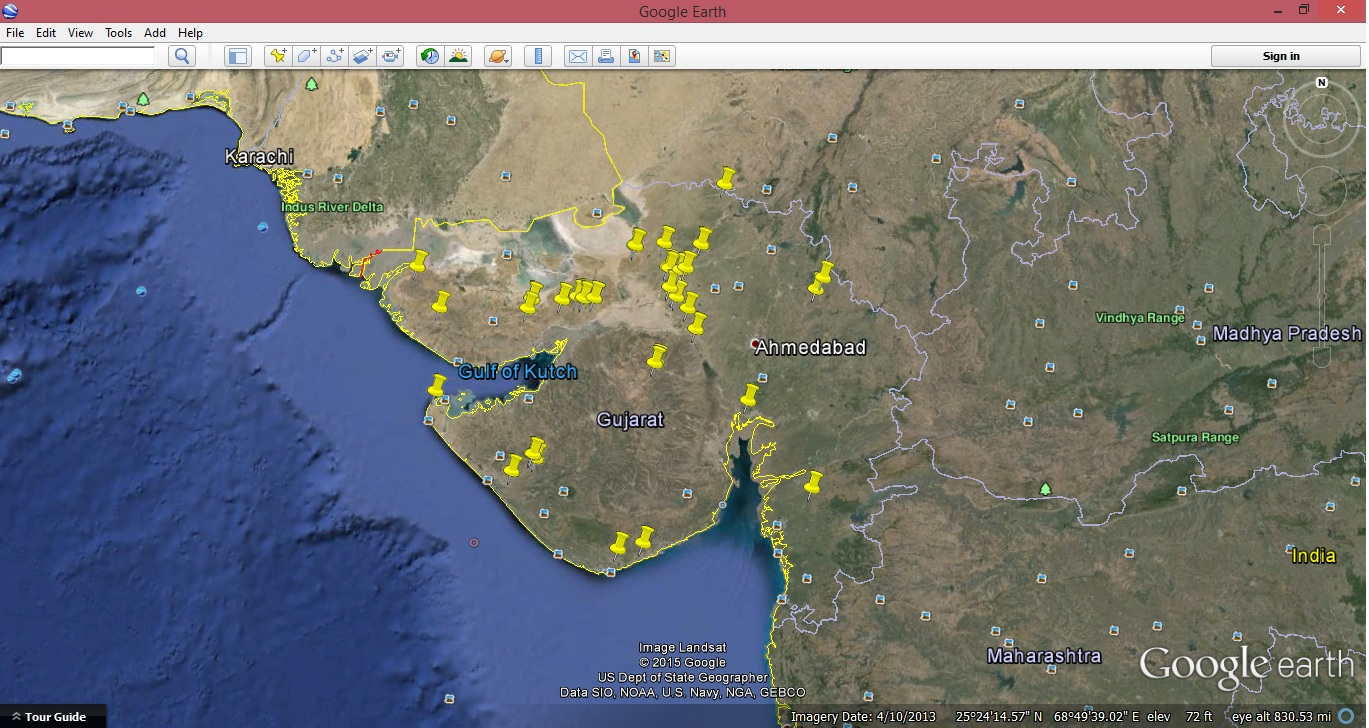
\includegraphics[scale=0.5]{GoogleEarthGuj}
\caption{Google Earth View of Solar PV Plants \geq 5MW in Gujarat}
\label{figc2h1} %% to refer use, \ref{}
\end{figure}
\\
The Fig \ref{figc2h2} gives the monthly solar energy generated by the PV plants given in Table \ref{tabc2h1} for four years from 2012 till August, 2015.
\\
\begin{figure}[H]
\centering
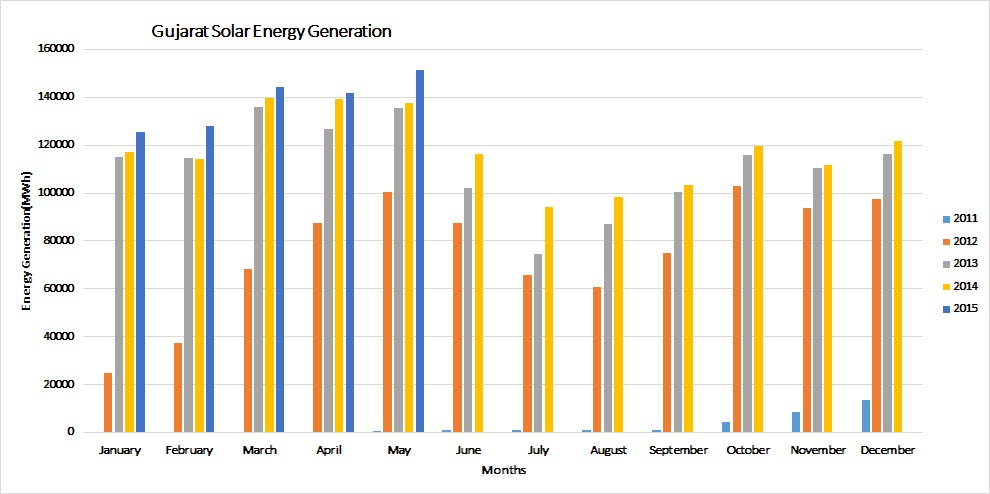
\includegraphics[scale=0.65]{Guj1}
\caption{Monthly Solar Power Generation in Gujarat as of Aug 2015}
\label{figc2h2} %% to refer use, \ref{}
\end{figure}
\\
The Capacity Utilization Factor (CUF)is very good measure of the efficiency of any power plant. The CUF of the entire generating capacity of PV plants in Table  \ref{tabc2h1} is calculated and presented in Fig.\ref{figc2h3}, which shows a rising efficiency of PV Power Plants in Gujarat over the course of 4 years.
\\

\begin{figure}[H]
\centering
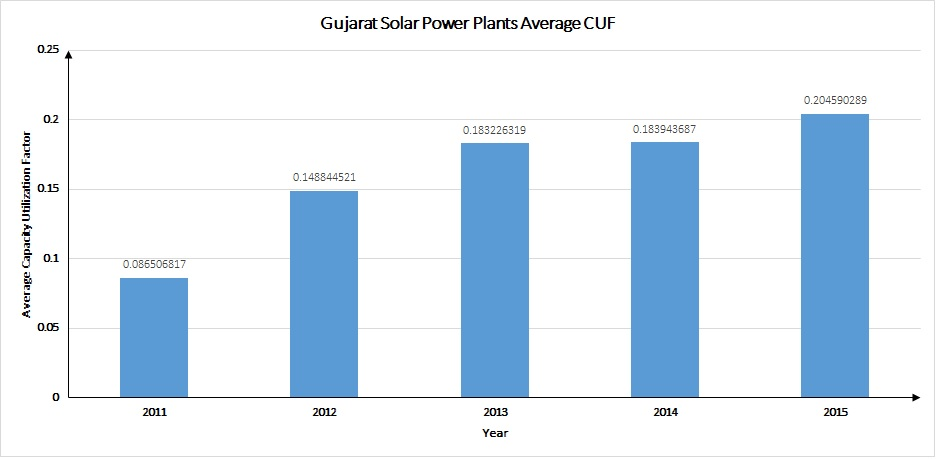
\includegraphics[scale=0.65]{Guj2}
\caption{Capacity Utilization Factor (CUF) for entire Gujarat}
\label{figc2h3} %% to refer use, \ref{}
\end{figure}

\newpage

\section{District-Wise Solar Energy Generation in Gujarat}
\
\
\
\
The data belonging to the Solar Plants in Fig \ref{tabc2h1} is segregated district-wise, it gives some really good insights. The Table \ref{tabc2h2} contains the capacity, average yearly energy generation, average yearly CUF and average yearly MWh/MW data.
\\ 
\begin{table}[H]
  \centering
%%From Excet to LATEX Add-In  
\caption{Gujarat District-Wise Solar Energy Data}
    \begin{tabular}{|r|c|c|r|r|}
    \hline
       & \textbf{Allotted,MW} & \textbf{CUF} & \multicolumn{1}{c|}{\textbf{Energy/Year}} & \multicolumn{1}{c|}{\textbf{MWh/MW}} \bigstrut\\
    \hline
    \textbf{Amreli} & 10 & 0.174114 & 9360.5402 & 936.054 \bigstrut\\
    \hline
    \textbf{Anand} & 15 & 0.147882 & 15591.016 & 1039.401 \bigstrut\\
    \hline
    \textbf{Banaskantha} & 55 & 0.18076 & 61724.444 & 1122.263 \bigstrut\\
    \hline
    \textbf{Jamnagar} & 25 & 0.162181 & 29841.603 & 1193.664 \bigstrut\\
    \hline
    \textbf{Junagadh} & 10 & 0.173891 & 11885.173 & 1188.517 \bigstrut\\
    \hline
    \textbf{Kutch} & 129 & 0.160941 & 132019.11 & 1023.404 \bigstrut\\
    \hline
    \textbf{Patan} & 397.5 & 0.166076 & 308645.3 & 776.4662 \bigstrut\\
    \hline
    \textbf{Porbandar} & 45 & 0.150004 & 49970.088 & 1110.446 \bigstrut\\
    \hline
    \textbf{Rajkot} & 60 & 0.165073 & 57596.477 & 959.9413 \bigstrut\\
    \hline
    \textbf{Sabarkantha} & 15 & 0.162073 & 17215.268 & 1147.685 \bigstrut\\
    \hline
    \textbf{Surat} & 5  & 0.14309 & 5229.0196 & 1045.804 \bigstrut\\
    \hline
    \textbf{Surendranagar} & 195 & 0.14968 & 177200.73 & 908.7217 \bigstrut\\
    \hline
    \textbf{Vadodara} & 10 & 0.064522 & 1009.5442 & 100.9544 \bigstrut\\
    \hline
    \end{tabular}%

%% All above Code is copied from Excel to LATEX Add-In 
    %\caption{Add caption}
    \label{tabc2h2}%

\end{table}
\\
The Fig \ref{figc2h4} shows the district-wise solar energy generation in gujarat. We can see that Patan leads all the districts in energy production (due to largest number of solar plants ) whereas Vadodara has the lowest energy production.
\\

\begin{figure}[H]
\centering
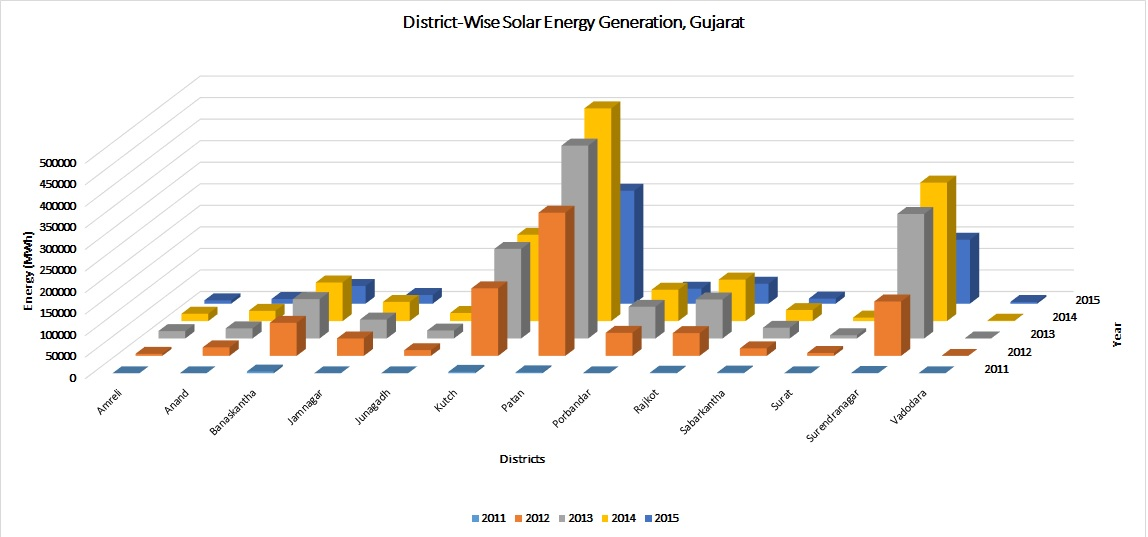
\includegraphics[scale=0.65]{Dist2}
\caption{District-Wise Solar Energy Generation in Gujarat}
\label{figc2h4} %% to refer use, \ref{}
\end{figure}
\\
The Fig \ref{figc2h5} shows the district-wise MWh/MW, it is also a good indicator of the efficiency of the solar power produced. We can see that over the years these values for each state have increased and Junagadh shows the highest MWh/MW value, while Patan shows the lowest MWh/MW value.
\\

\begin{figure}[H]
\centering
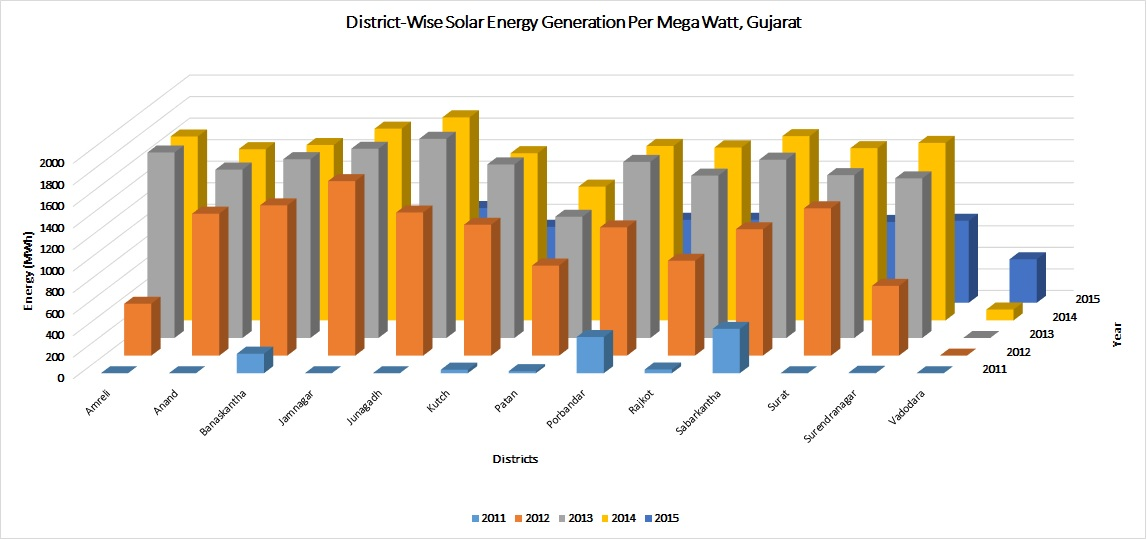
\includegraphics[scale=0.65]{Dist3}
\caption{District-Wise MWh/MW in Gujarat}
\label{figc2h5} %% to refer use, \ref{}
\end{figure}
\\
The Fig \ref{figc2h6} shows the district-wise CUF in Gujarat. We can see that similar to the last graph here to Junagadh has the highest value and Patan has the lowest value. We can say that CUF and MWh/MW have a good correlation, and they show efficiency of energy generation in different ways but of similar forms.
\\

\begin{figure}[H]
\centering
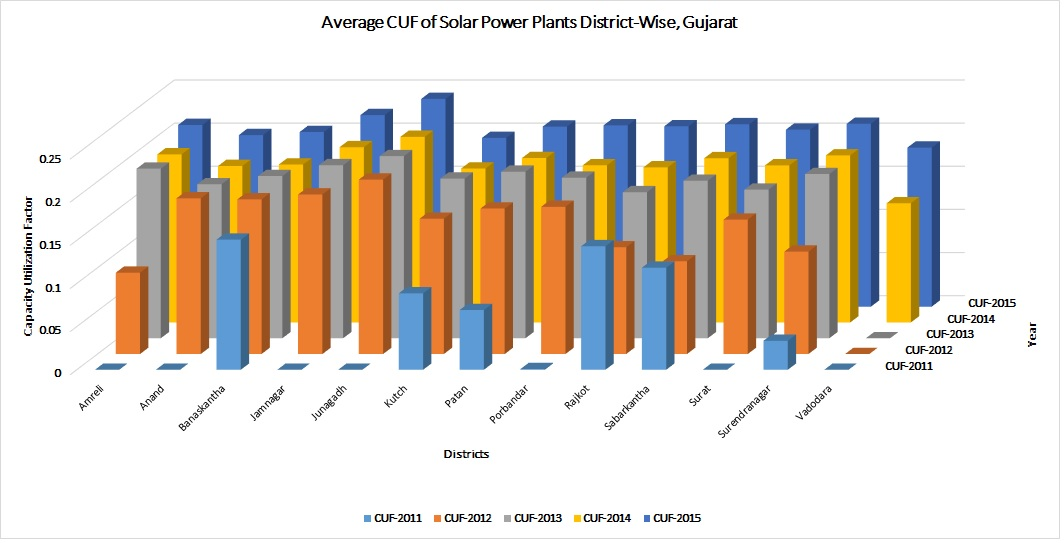
\includegraphics[scale=0.65]{Dist1}
\caption{District-Wise Capacity Utilization Factor (CUF) in Gujarat}
\label{figc2h6} %% to refer use, \ref{}
\end{figure}

\section{Charanka Solar Park Analysis on the basis of PV Technology}
\
\
\
\
Charanka Solar Park in Patan district is Gujarat's largest Solar park as of August, 2015 with eighteen solar power plants and a total capacity of 272MW. Models of all the eighteen solar plants were simulated in PVsyst software and an analysis of performance of Mono-Crystalline (Mono), Poly-Crystalline (Poly) and Thin Film (Thin) PV technologies has been carried out. The Table \ref{tabc2h3} gives the results of that analysis values which have a letter P after them are simulated quantities and others are real quantities.
\\
\begin{table}[H]
  \centering
  \caption{Charaka Solar Park Analysis}
%%From Excet to LATEX Add-In  
    \begin{tabular}{|c|l|l|l|l|l|l|}
    \hline
    \textbf{} & \textbf{Name} & \textbf{MW} & \textbf{MWh} & {\textbf{MWh P}} & \textbf{MWh/MW} & \textbf{MWh/MW P} \bigstrut\\
    \hline
    \textbf{Mono} & LANCO  & 15.0 & 20506.3 & 27379.0 & 1367.1 & 1825.3 \bigstrut\\
\cline{2-7}       & \textbf{Tot Energy} & \textbf{15.0} & \textbf{20506.3} & \textbf{27379.0} &    &  \bigstrut\\
\cline{2-7}       & \textbf{MWh/MW} &    & \textbf{1367.1} & \textbf{1825.3} &    &  \bigstrut\\
\cline{2-7}       & \textbf{Average} &    &    &    & \textbf{1367.1} & \textbf{1825.3} \bigstrut\\
    \hline
    \textbf{Poly } & GSPC  & 5.0 & 8906.5 & 8358.0 & 1781.3 & 1671.6 \bigstrut\\
\cline{2-7}       & Surana  & 5.0 & 7899.3 & 9053.0 & 1579.9 & 1810.6 \bigstrut\\
\cline{2-7}       & NKG  & 10.0 & 17729.4 & 17168.0 & 1772.9 & 1716.8 \bigstrut\\
\cline{2-7}       & GMR  & 25.0 & 42603.7 & 44041.0 & 1704.1 & 1761.6 \bigstrut\\
\cline{2-7}       & Sun Edison & 25.0 & 42255.0 & 43728.0 & 1690.2 & 1749.1 \bigstrut\\
\cline{2-7}       & Emami  & 10.0 & 16958.8 & 17954.0 & 1695.9 & 1795.4 \bigstrut\\
\cline{2-7}       & GPCL & 5.0 & 7952.3 & 8863.0 & 1590.5 & 1772.6 \bigstrut\\
\cline{2-7}       & Palace & 15.0 & 26336.3 & 26946.0 & 1755.8 & 1796.4 \bigstrut\\
\cline{2-7}       & Avtar  & 5.0 & 8117.1 & 8611.0 & 1623.4 & 1722.2 \bigstrut\\
\cline{2-7}       & Torrent  & 51.0 & 77483.7 & 89184.0 & 1519.3 & 1748.7 \bigstrut\\
\cline{2-7}       & \textbf{Tot Energy} & \textbf{156.0} & \textbf{256241.9} & \textbf{273906.0} &    &  \bigstrut\\
\cline{2-7}       & \textbf{MWh/MW} &    & \textbf{1642.6} & \textbf{1755.8} &    &  \bigstrut\\
\cline{2-7}       & \textbf{Average} &    &    &    & \textbf{1671.3} & \textbf{1754.5} \bigstrut\\
    \hline
    \textbf{Thin} & Alex  & 25.0 & 41968.2 & 47372.0 & 1678.7 & 1894.9 \bigstrut\\
\cline{2-7}       & ZF  & 5.0 & 8734.6 & 8722.0 & 1746.9 & 1744.4 \bigstrut\\
\cline{2-7}       & Sun Clean & 6.0 & 10265.9 & 10408.0 & 1711.0 & 1734.7 \bigstrut\\
\cline{2-7}       & Solarified & 20.0 & 34091.4 & 36212.0 & 1704.6 & 1810.6 \bigstrut\\
\cline{2-7}       & AES  & 15.0 & 23241.9 & 26368.0 & 1549.5 & 1757.9 \bigstrut\\
\cline{2-7}       & Roha  & 25.0 & 43540.3 & 47860.0 & 1741.6 & 1914.4 \bigstrut\\
\cline{2-7}       & Yantra & 5.0 & 6981.4 & 8858.0 & 1396.3 & 1771.6 \bigstrut\\
\cline{2-7}       & \textbf{Tot Energy} & \textbf{101.0} & \textbf{168823.7} & \textbf{185800.0} &    &  \bigstrut\\
\cline{2-7}       & \textbf{MWh/MW} &    & \textbf{1671.5} & \textbf{1839.6} &    &  \bigstrut\\
\cline{2-7}       & \textbf{Average} &    &    &    & \textbf{1650.0} & \textbf{1804.1} \bigstrut\\
    \hline
    \end{tabular}%

%% All above Code is copied from Excel to LATEX Add-In 
    %\caption{Add caption}
    \label{tabc2h3}%

\end{table}
\\
The Fig \ref{figc2h7} represents the PV Technology wise solar energy generation. We can see that Poly is highest generation as most of the plants employ Poly and as only one plant uses Mono it gives the lowest generation. But, this is not an actual measurement of performance of the PV Technologies.
\\

\begin{figure}[H]
\centering
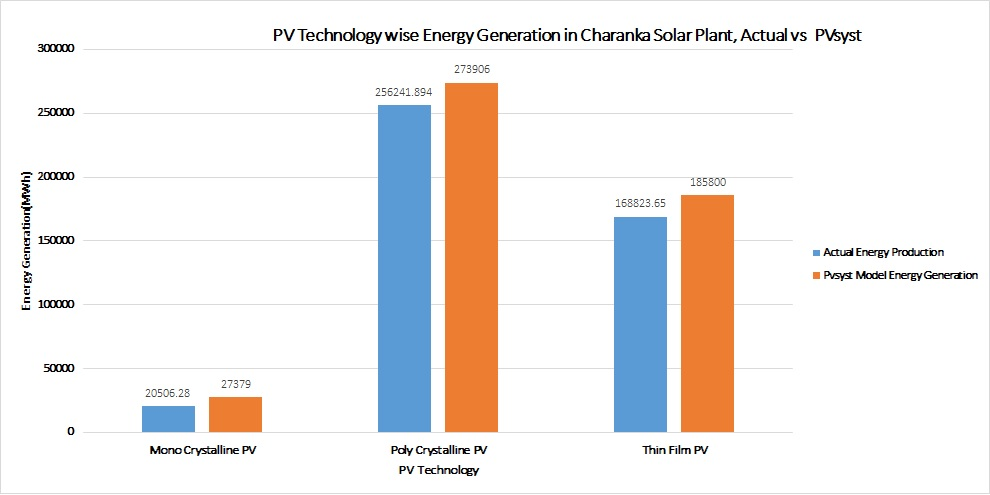
\includegraphics[scale=0.5]{Charanka2}
\caption{Charanka Solar Park PV Technology-Wise Energy Generation}
\label{figc2h7} %% to refer use, \ref{}
\end{figure}
\\
The Fig \ref{figc2h8} gives a good measure of performance of the different PV Technologies used in Charanka Solar Park, by measuring MWh/MW for all the plants using the same PV technology as a whole. We can see that with actual data Poly performs best and Mono performs the worst, however when we consider simulated values Mono performs best and Poly performs worst. 
\\

\begin{figure}[H]
\centering
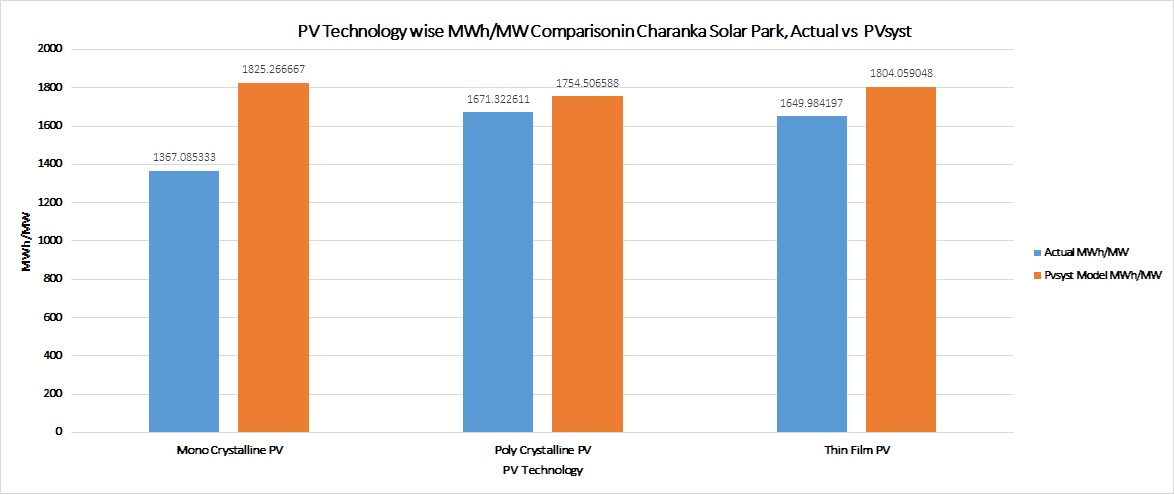
\includegraphics[scale=0.5]{Charanka1}
\caption{Charanka Solar Park PV Technology-Wise MWh/MW Comparison}
\label{figc2h8} %% to refer use, \ref{}
\end{figure}
\\
The Fig \ref{figc2h9} shows the PV Technology wise CUF comparison of Charanka Solar Park. We can observe that the the real and simulated values of CUF for Poly and Thin are approximately equal validating the PVsyst models, however even in this graph the simulated values for Mono are fairly larger than the real values; which indicates some modeling error.(most probably error could be the generalised weather data which PVsyst produces) 
\\
\begin{figure}[H]
\centering
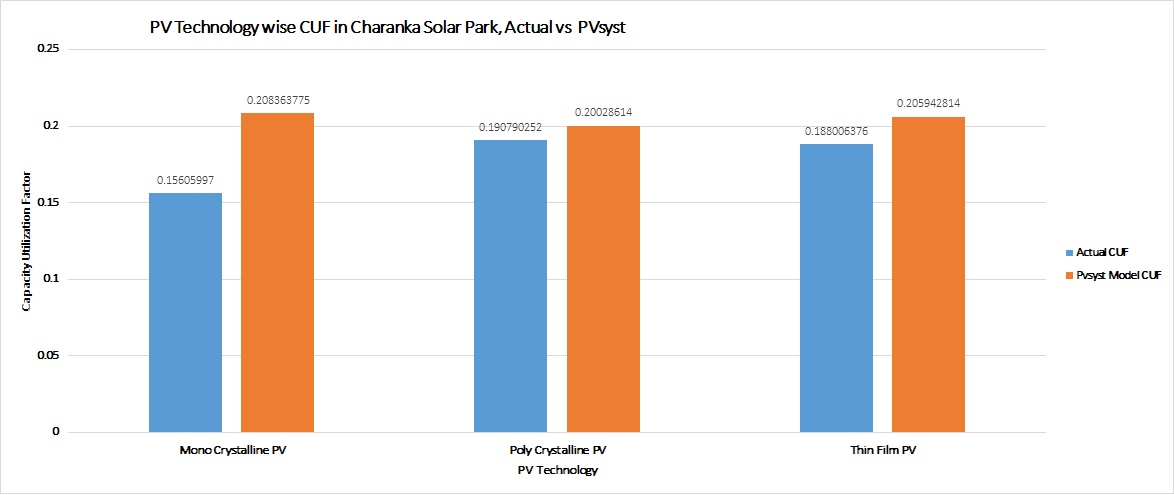
\includegraphics[scale=0.5]{Charanka3}
\caption{Charanka Solar Park PV Technology-Wise CUF Comparison}
\label{figc2h9} %% to refer use, \ref{}
\end{figure}

\section{Tracking Mechanism Performance Assessment using BACKBONE Plant Data}
\
\
\
\
The BACKBONE Enterprise LTD, 5MW Solar PV plant, in Kutch district is the only plant in whole of Gujarat to have a tracking mechanism. It uses a Single Axis (N-S axis)tracker system, details of which are given in Table \ref{tabc2h4}.
\\
\begin{table}[H]
  \centering
%%From Excet to LATEX Add-In  
    \begin{tabular}{|l|l|}
    \hline
    \textbf{Make} & SUNLINK  ViaSol Tracker \\
    \hline
    \textbf{Tracking Type (East/West)} & One-Axis Horizontal \\
    \hline
    \textbf{Tilt-Range} & +/- 45º (maximum) \\
    \hline
    \textbf{Backtracking} & Yes, Standard \\
    \hline
    \textbf{Sub-Array Rated Power} & Up to 1 MW dc \\
    \hline
    \textbf{Wind Load Capacity} & Up to 150 mph (35 mph stow) \\
    \hline
    \textbf{Time to Stow or Recover} & Less than 2 minutes \\
    \hline
    \textbf{Tracking Method} & Based on NASA time-and-location algorithm \\
    \hline
    \textbf{Drive Type} & Fluid Power \\
    \hline
    \textbf{Controller} & PLC controller utilizing industrial automation components \\
    \hline
    \textbf{Power Supply} & AC Supply from Auxiliary \\
    \hline
    \end{tabular}
%% All above Code is copied from Excel to LATEX Add-In 
    \caption{Tracker System Specifications}
    \label{tabc2h4}
\end{table}
\\
A model of the plant was created in PVsyst and simulated for Fixed Tilt (FT), Seasonal Tilt (ST), and Dual Axis Tracker (DA). We had the real values for the Single Axis Tracker (SA) and then compared them for analysis. The Table \ref{tabc2h5} shows the result of the PVsyst software simulation. 
\\

\begin{table}[H]
  \centering
     \caption{Tracker System Performance Comparison in PVsyst}
%%From Excet to LATEX Add-In  
    \begin{tabular}{|r|r|r|r|r|r|}
    \hline
    \textbf{} & \textbf{Actual} & \textbf{Fixed Tilt} & \textbf{Seasonal Tilt} & \textbf{N-S Axis} & \textbf{Dual-Axes} \\
    \hline
    \textbf{January} & 552.129 & 881.9 & 979.6 & 905   & 1174 \\
    \hline
    \textbf{February} & 642.4595 & 764.6 & 788.2 & 826   & 967 \\
    \hline
    \textbf{March} & 865.858 & 962.3 & 907.9 & 1144  & 1240 t\\
    \hline
    \textbf{April} & 916.5298 & 876   & 884   & 1143  & 1186 \\
    \hline
    \textbf{May} & 1044.885 & 863.4 & 883.2 & 1182  & 1209 \\
    \hline
    \textbf{June} & 599.0633 & 754.6 & 775.4 & 1020  & 1041 \\
    \hline
    \textbf{July} & 435.0063 & 581.8 & 595   & 730   & 740 \\
    \hline
    \textbf{August} & 425.8848 & 567.2 & 575.6 & 676   & 685 \\
    \hline
    \textbf{September} & 486.5465 & 741   & 741   & 874   & 920 \\
    \hline
    \textbf{October} & 550.0673 & 870.3 & 875.3 & 995   & 1136 \\
    \hline
    \textbf{November} & 452.825 & 797.9 & 864   & 825   & 1032 \\
    \hline
    \textbf{December} & 459.0528 & 825.4 & 932.2 & 812   & 1090 \\
    \hline
          &       &       &       &       &  \\
    \hline
    \textbf{Total Energy} & 7430.307 & 9486.4 & 9801.4 & 11132 & 12420 \\
    \hline
    \textbf{} &       &       &       &       &  \\
    \hline
    \textbf{MWh/MW} & 1486.061 & 1897.28 & 1960.28 & 2226.4 & 2484 \\
    \hline
          &       &       &       &       &  \\
    \hline
    \textbf{CUF} & 0.169642 & 0.216584 & 0.223776 & 0.254155 & 0.283562 \\
    \hline
    \end{tabular}%
    %% All above Code is copied from Excel to LATEX Add-In 
 
    \label{tabc2h5}%
\end{table}
\\
The Fig \ref{figc2h10} shows the monthly solar generations for different types of tracking mechanisms, and we see that the Dual Axis Tracker gives the best performance while Fixed Tilt gives the worst.
\\
\begin{figure}[H]
\centering
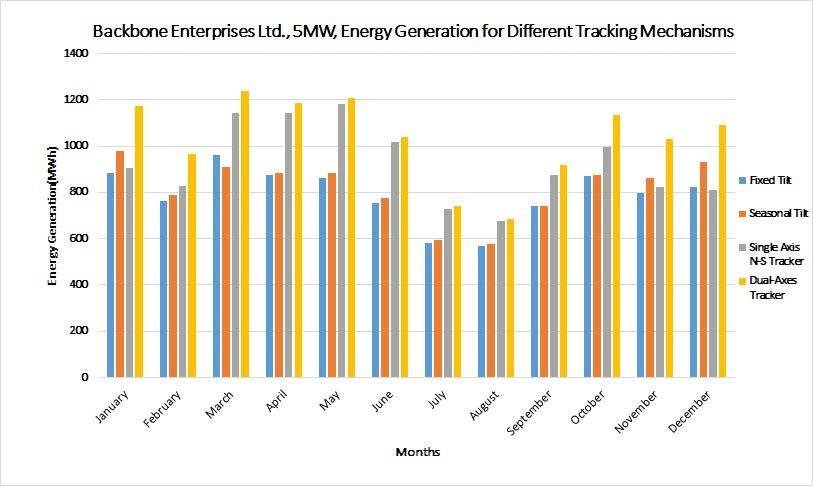
\includegraphics[scale=0.75]{Backbone1}
\caption{Monthly Solar Generation Comparison of different Tracking Mechanisms}
\label{figc2h10} %% to refer use, \ref{}
\end{figure}
\\
The Fig \ref{figc2h11} represents the CUF comparison of different tracking mechanisms. We observe that the performance of FT, ST, SA and DA improves in this same order.

\\

\begin{figure}[H]
\centering
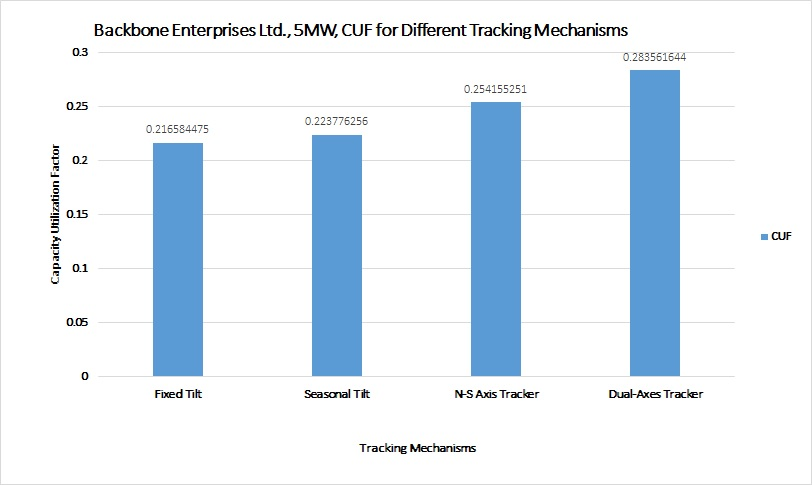
\includegraphics[scale=0.65]{Backbone3}
\caption{CUF Comparison of different Tracking Mechanisms}
\label{figc2h11} %% to refer use, \ref{}
\end{figure}

\newpage

\section{Generation and Weather Data Resources}
\
\
\
\
The historical generation data can be sort from SLDC, but it has a resolution of one day. To get higher resolution generation data of the order of days or hours, we have to take it directly from the Solar PV Plant SCADA system. But in most of the cases the plant logs only daily data for saving memory of the SCADA systems. I have collected generation data from the BACKBONE plant at a daily resolution.\\

Similarly historical weather data is available at Meteorological Institutes Website, they will usually have data at almost all resolutions, but you will have to pay for the data. Also, some web linked softwares like Meteonorm alsso provide quality weather data at almost all resolutions at a fee. However, the data obtained from these sources would not be cent percent accurate for the exact plant location. Hence, weather data logged into the plant SCADA system is the most reliable weather data we can ever get. I have received only Global Horizoltal Radiation (GHI) from Backbone as there is no provision for temperature and wind speed logging.



